
% LaTeX Beamer file automatically generated from Doconce
% http://code.google.com/p/doconce

%-------------------- begin preamble ----------------------

\documentclass{beamer}

\usetheme{default}
\usecolortheme{default}

% turn off the almost invisible, yet disturbing, navigation symbols:
\setbeamertemplate{navigation symbols}{}

% Examples on customization:
%\usecolortheme[named=RawSienna]{structure}
%\usetheme[height=7mm]{Rochester}
%\setbeamerfont{frametitle}{family=\rmfamily,shape=\itshape}
%\setbeamertemplate{items}[ball]
%\setbeamertemplate{blocks}[rounded][shadow=true]
%\useoutertheme{infolines}
%
%\usefonttheme{}
%\useinntertheme{}
%
%\setbeameroption{show notes}
%\setbeameroption{show notes on second screen=right}

% fine for B/W printing:
%\usecolortheme{seahorse}

\usepackage{pgf,pgfarrows,pgfnodes,pgfautomata,pgfheaps,pgfshade}
\usepackage{graphicx}
\usepackage{epsfig}
\usepackage{fancyvrb,relsize}
\usepackage{amsmath,amssymb,bm}
%\usepackage[latin1]{inputenc}
\usepackage[utf8]{inputenc}
\usepackage{colortbl}
\usepackage[english]{babel}
\usepackage{tikz}
\usepackage{framed,anslistings}
% Use some nice templates
\beamertemplatetransparentcovereddynamic

% Delete this, if you do not want the table of contents to pop up at
% the beginning of each section:
\AtBeginSection[]
{
    \begin{frame}<beamer>[plain]
    \frametitle{}
    \tableofcontents[currentsection]
    \end{frame}
}

% Delete this, if you do not want the table of contents to pop up at
% the beginning of each section:
\AtBeginSection[]
{
    \begin{frame}<beamer>[plain]
    \frametitle{}
    \tableofcontents[currentsection]
    \end{frame}
}

% If you wish to uncover everything in a step-wise fashion, uncomment
% the following command:

%\beamerdefaultoverlayspecification{<+->}

\newcommand{\shortinlinecomment}[3]{\note{\textbf{#1}: #2}}
\newcommand{\longinlinecomment}[3]{\shortinlinecomment{#1}{#2}{#3}}

\newenvironment{notice_colors1admon}[1][]{\begin{block}{#1}}{\end{block}}
\newenvironment{notice_colors2admon}[1][]{\begin{block}{#1}}{\end{block}}
\newenvironment{notice_graybox3admon}[1][]{\begin{block}{#1}}{\end{block}}
\newenvironment{notice_yellowboxadmon}[1][]{\begin{block}{#1}}{\end{block}}
\newenvironment{summary_colors1admon}[1][]{\begin{block}{#1}}{\end{block}}
\newenvironment{summary_colors2admon}[1][]{\begin{block}{#1}}{\end{block}}
\newenvironment{summary_graybox3admon}[1][]{\begin{block}{#1}}{\end{block}}
\newenvironment{summary_yellowboxadmon}[1][]{\begin{block}{#1}}{\end{block}}
\newenvironment{warning_colors1admon}[1][]{\begin{block}{#1}}{\end{block}}
\newenvironment{warning_colors2admon}[1][]{\begin{block}{#1}}{\end{block}}
\newenvironment{warning_graybox3admon}[1][]{\begin{block}{#1}}{\end{block}}
\newenvironment{warning_yellowboxadmon}[1][]{\begin{block}{#1}}{\end{block}}
\newenvironment{question_colors1admon}[1][]{\begin{block}{#1}}{\end{block}}
\newenvironment{question_colors2admon}[1][]{\begin{block}{#1}}{\end{block}}
\newenvironment{question_graybox3admon}[1][]{\begin{block}{#1}}{\end{block}}
\newenvironment{question_yellowboxadmon}[1][]{\begin{block}{#1}}{\end{block}}
\newenvironment{block_colors1admon}[1][]{\begin{block}{#1}}{\end{block}}
\newenvironment{block_colors2admon}[1][]{\begin{block}{#1}}{\end{block}}
\newenvironment{block_graybox3admon}[1][]{\begin{block}{#1}}{\end{block}}
\newenvironment{block_yellowboxadmon}[1][]{\begin{block}{#1}}{\end{block}}
\newenvironment{paragraphadmon}[1][]{\begin{block}{#1}}{\end{block}}
\newenvironment{graybox1admon}[1][]{\begin{block}{#1}}{\end{block}}
\newenvironment{graybox2admon}[1][]{\begin{block}{#1}}{\end{block}}
\newcommand{\grayboxhrules}[1]{\begin{block}{}#1\end{block}}



% insert custom LaTeX commands...

\makeindex

%-------------------- end preamble ----------------------

\begin{document}


\renewcommand{\u}{\pmb{u}}

\newcommand{\xbm}{\bm{x}}
\newcommand{\normalvecbm}{\bm{n}}
\newcommand{\ubm}{\bm{u}}


\newcommand{\x}{\pmb{x}}
\newcommand{\normalvec}{\pmb{n}}
\newcommand{\Ddt}[1]{\frac{D#1}{dt}}
\newcommand{\halfi}{1/2}
\newcommand{\half}{\frac{1}{2}}
\newcommand{\report}{test report}


% ------------------- main content ----------------------



% ----------------- title -------------------------
\title{On the Technicalities of Scientific Writing Anno 2012: The Doconce Way}

% ----------------- author(s) -------------------------
\author{Hans Petter Langtangen\inst{1,2}}
\institute{Simula Research Laboratory\inst{1}
\and
University of Oslo\inst{2}}
% ----------------- end author(s) -------------------------


\date{Jun 29, 2013
% <titlepage figure>
}

\begin{frame}[plain,fragile]
\titlepage
\end{frame}

\begin{frame}[plain,fragile]
\frametitle{Figure and bullet list}

\begin{columns}
\column{0.35\textwidth}

\pause
\begin{block}{}
\begin{itemize}
  \item Here is a \emph{wave packet}

  \item It can move

  \item But here it is just a figure
\end{itemize}

\noindent
\end{block}


\column{0.65\textwidth}
\begin{center}  % inline figure
  \centerline{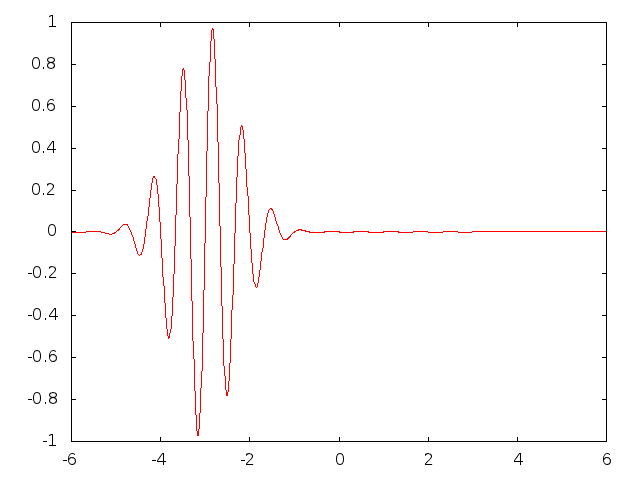
\includegraphics[width=0.9\linewidth]{../doc/manual/figs/wavepacket_0001.png}}
\end{center}


\end{columns}



% Test that it is okay to leave out width if there are only two columns




\pause
\begin{block}{}
Here we have a paragraph to pop up in red.
And a line more
\end{block}


\shortinlinecomment{hpl 1}{ Here are some notes that can go to notes typesetting
in the slide environment. }{ Here are some notes }

\note{
One can also have ordinary notes.
Over multiple lines.
}
\end{frame}

\begin{frame}[plain,fragile]
\frametitle{Scientific writing needs to address many new media}

\begin{itemize}
 \item<2-> Old days (1985-2005): mostly black-and-white documents aimed at printing

 \item<3-> Now: also color PDF, web pages, wikis - for paper, PC, iPad, ...

 \item<4-> {\LaTeX} writing may be very different from writing in other formats

 \item<5-> Main problem:
\begin{itemize}

    \item<6-> {\LaTeX} provide all sorts of fancy packages, but

    \item<7-> PDF in browsers has limited capabilities (design, navigation)
      compared to native HTML formats

\end{itemize}

\noindent
 \item<8-> Conclusion: We need more than {\LaTeX}
\end{itemize}

\noindent
\end{frame}

\begin{frame}[plain,fragile]
\frametitle{Some math and computer code}

\[ f(x,y,t) = e^{-xt}\sin\pi y \]
Python implementation:

\begin{Verbatim}[numbers=none,fontsize=\fontsize{9pt}{9pt},baselinestretch=0.95]
import numpy as np

def f(x, y, t):
    return np.exp(-x*t)*np.sin(np.pi*y)

class Fancy:
    def __init__(self):
        pass

    def __call__(self, x, y, t):
        return f(x, y, t)

f2 = Fancy()
\end{Verbatim}
\end{frame}

\begin{frame}[plain,fragile]
\frametitle{Admon blocks}

Can use admons to simulate blocks:


\begin{graybox1admon}[Key PDE:]
This box has title and math in normal 90 percent font:
\[ \frac{\partial u}{\partial t} = \nabla^2 u \]
\end{graybox1admon}


\pause
\begin{graybox1admon}[]
Just some block with text and a conclusion that something is important.
This one pops up after the rest of the slide.
\end{graybox1admon}



\begin{graybox1admon}[Warning.]
\vspace{0.5mm}\par\noindent
{\footnotesize Can use, e.g., a warning admon to have my own notes, preferably
inside preprocess/mako if statements to turn notes on and off.
This one is typeset in a small font and with the default
title (Warning) since no title is specified. \par}
\end{graybox1admon}
\end{frame}

\end{document}
